\section{Results}
\label{sec:results}

We organize the analysis around two complementary measurements that probe different aspects of the same representation. A linear probe asks whether a chemical property is \emph{encoded} as a readable signal in the residual stream---it locates information. A causal intervention along the probe's decision direction asks whether that direction is \emph{used} by the rest of the encoder---it tests function. We present probing in Section~\ref{sec:res-probe} and intervention in Section~\ref{sec:res-steer}, then synthesize them in Section~\ref{sec:res-disc}. We focus the main text on four representative properties---aromaticity, ring membership, degree, and chiral tag---that span the qualitatively distinct regimes we observe; the remaining four tasks fall into one of these regimes (Appendix~\ref{app:probe-all}). \xiaoyan{TODO: This should be about attention and probing}

\subsection{Linear probing: what is encoded}
\label{sec:res-probe}
\begin{figure*}[t]
\centering
\begin{subfigure}[t]{0.24\textwidth}
    \centering
    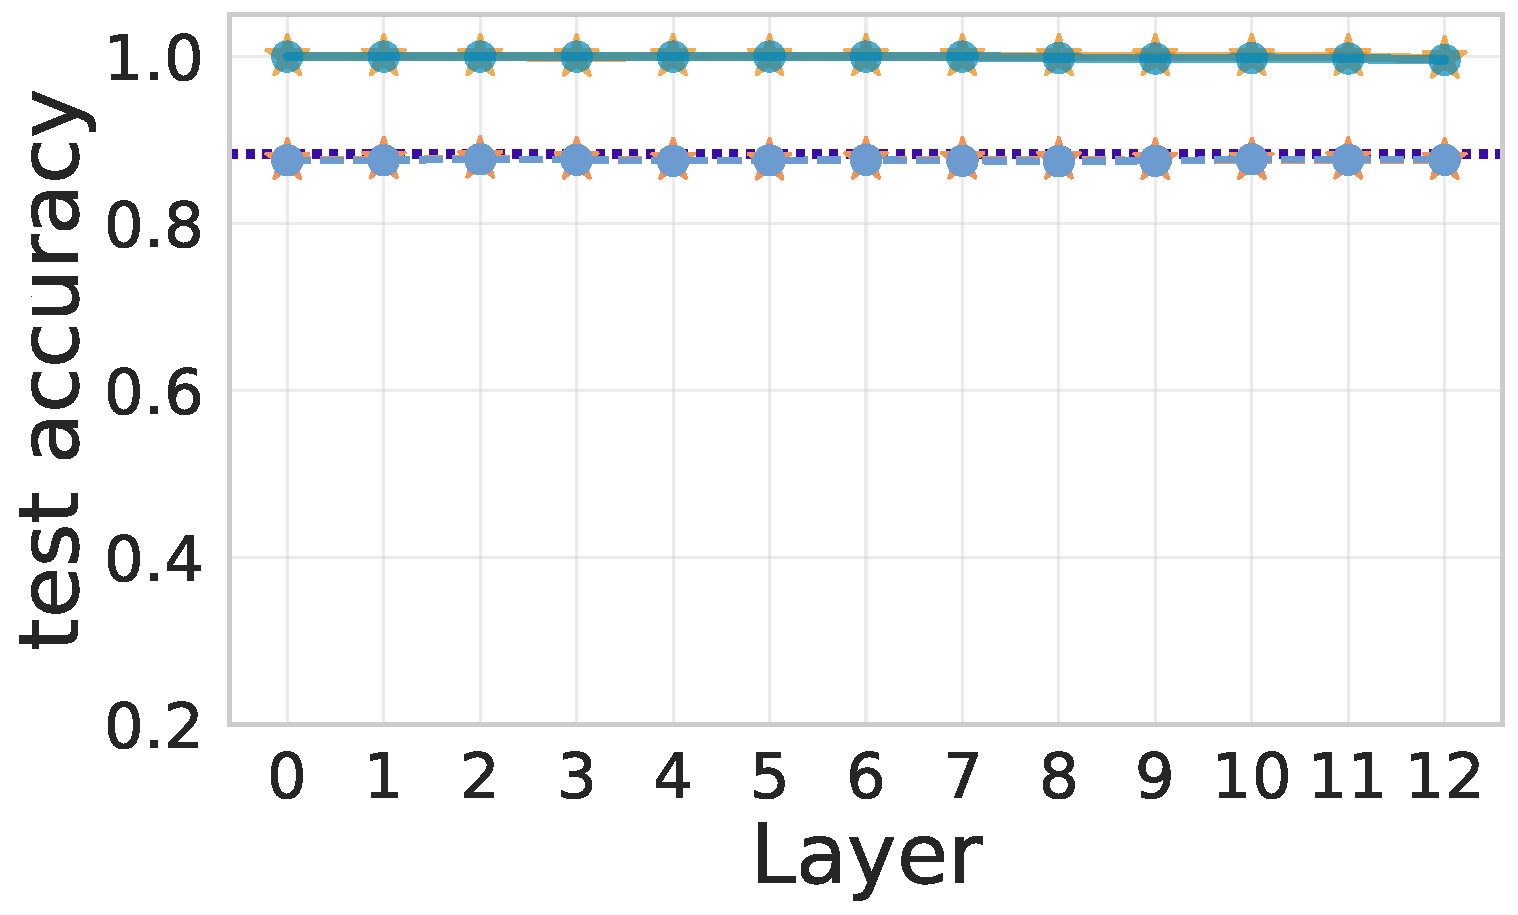
\includegraphics[width=\linewidth]{results_combined/is_aromatic.pdf}
    \subcaption{is aromatic}
    \label{fig:acc-is-aromatic}
\end{subfigure}\hfill
\begin{subfigure}[t]{0.24\textwidth}
    \centering
    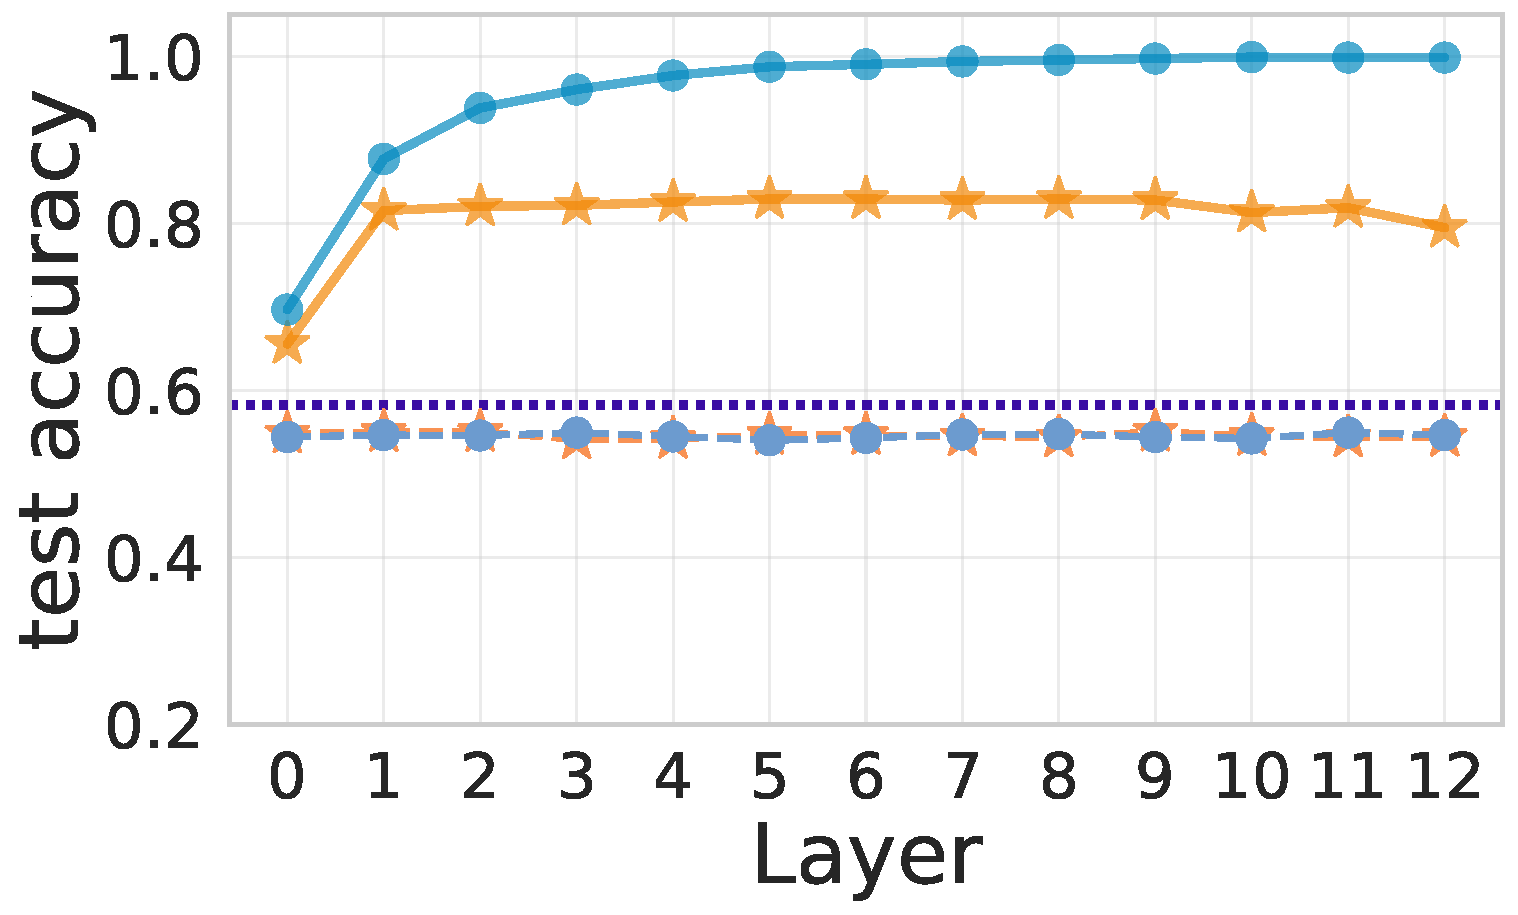
\includegraphics[width=\linewidth]{results_combined/is_in_ring.pdf}
    \subcaption{is in ring}
    \label{fig:acc-is-in-ring}
\end{subfigure}\hfill
\begin{subfigure}[t]{0.24\textwidth}
    \centering
    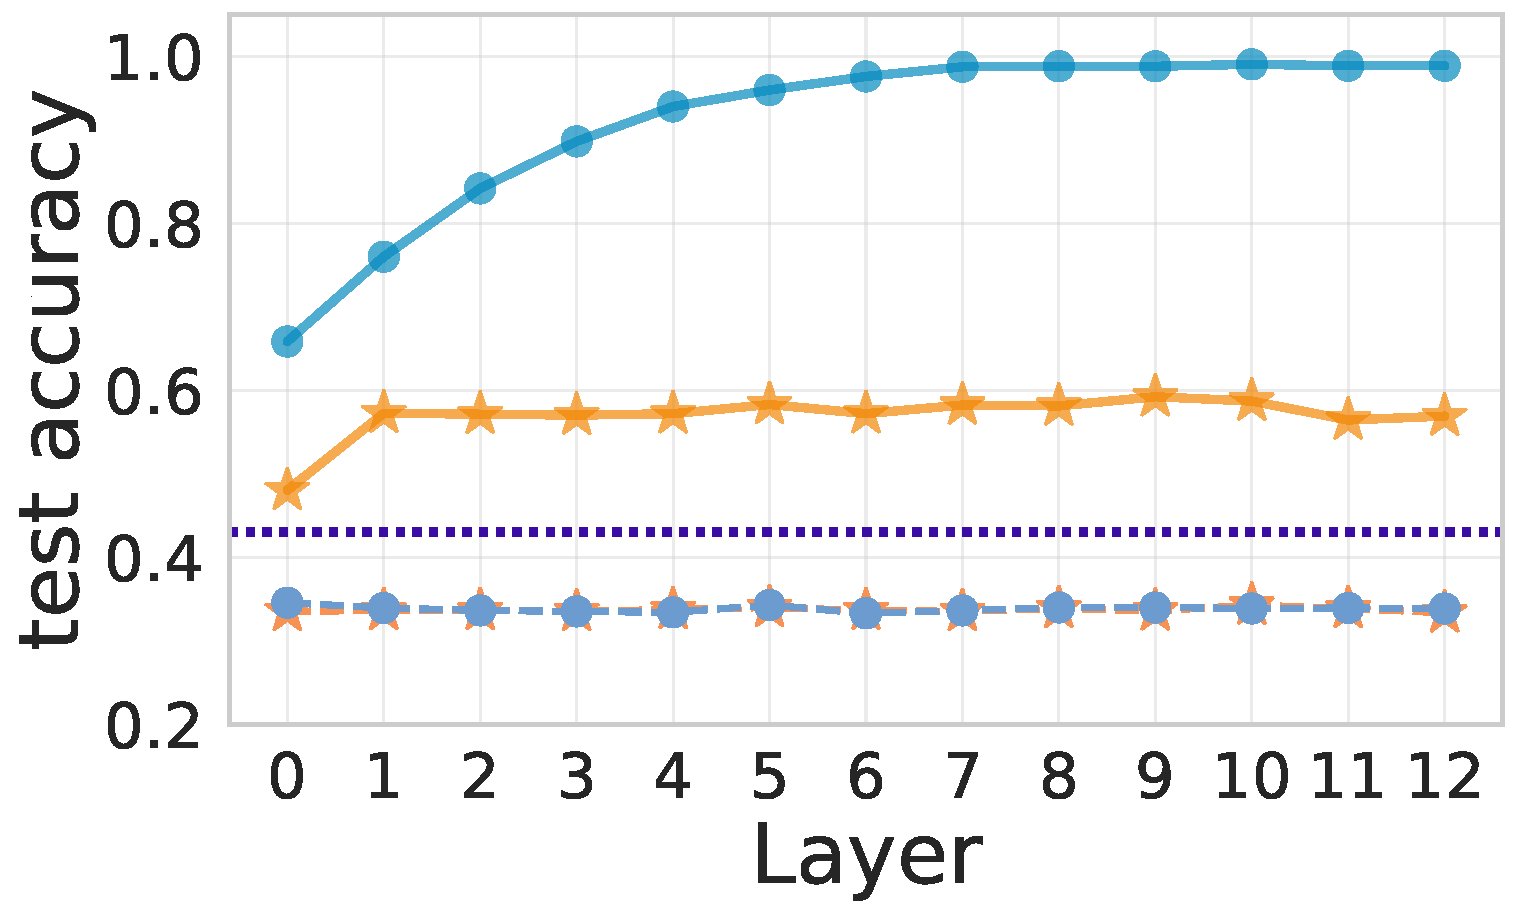
\includegraphics[width=\linewidth]{results_combined/degree.pdf}
    \subcaption{degree}
    \label{fig:acc-degree}
\end{subfigure}\hfill
\begin{subfigure}[t]{0.24\textwidth}
    \centering
    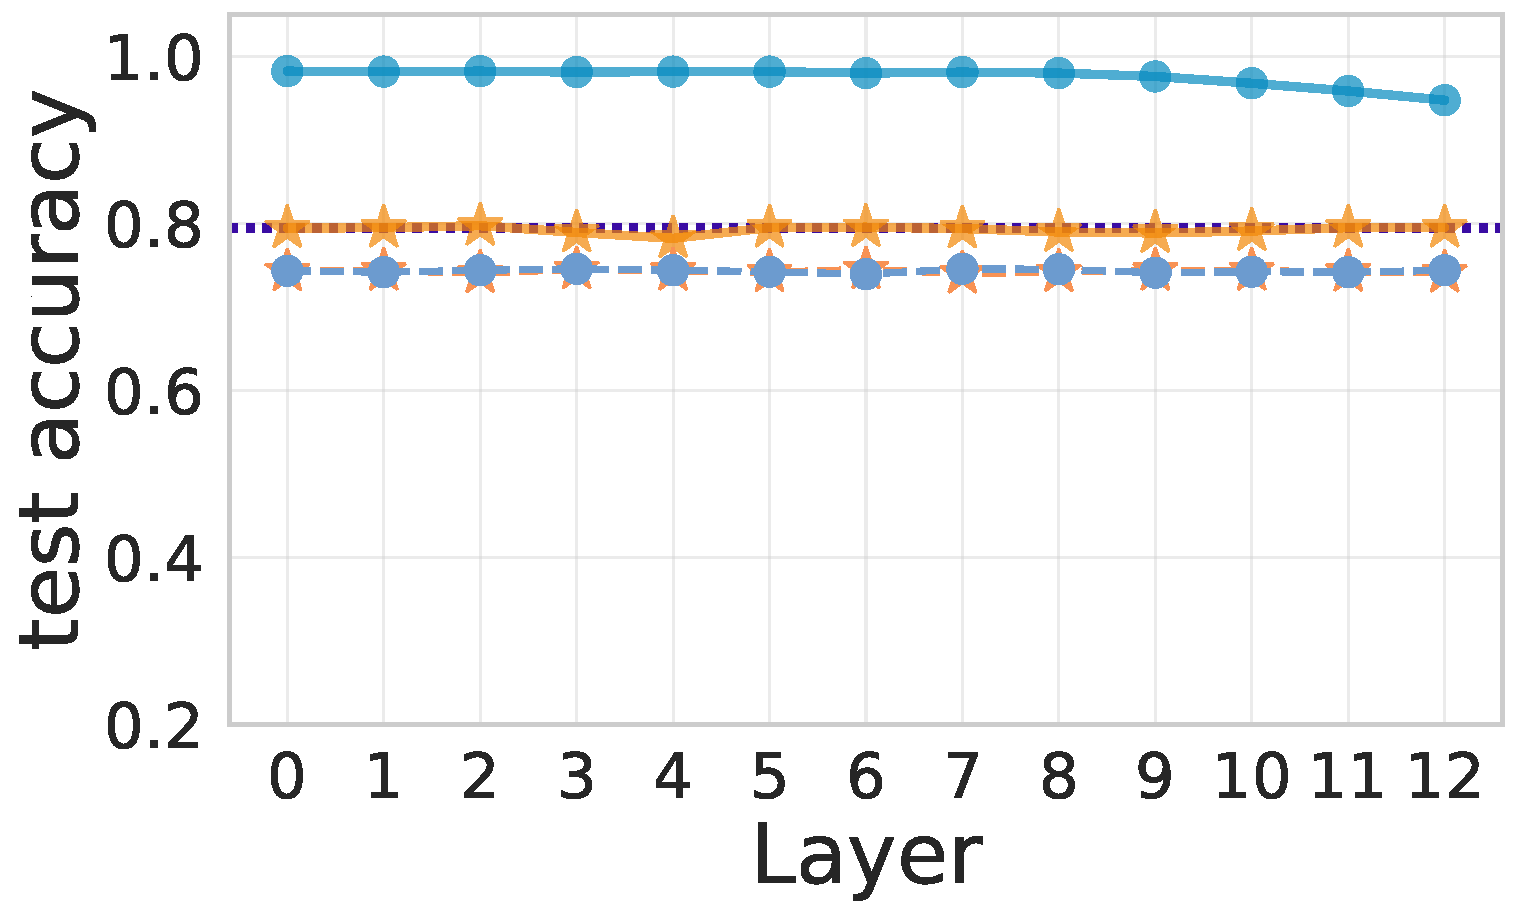
\includegraphics[width=\linewidth]{results_combined/chiral_tag.pdf}
    \subcaption{chiral tag}
    \label{fig:acc-chiral-tag}
\end{subfigure}

\vspace{0.4em}

\begin{subfigure}[t]{0.24\textwidth}
    \centering
    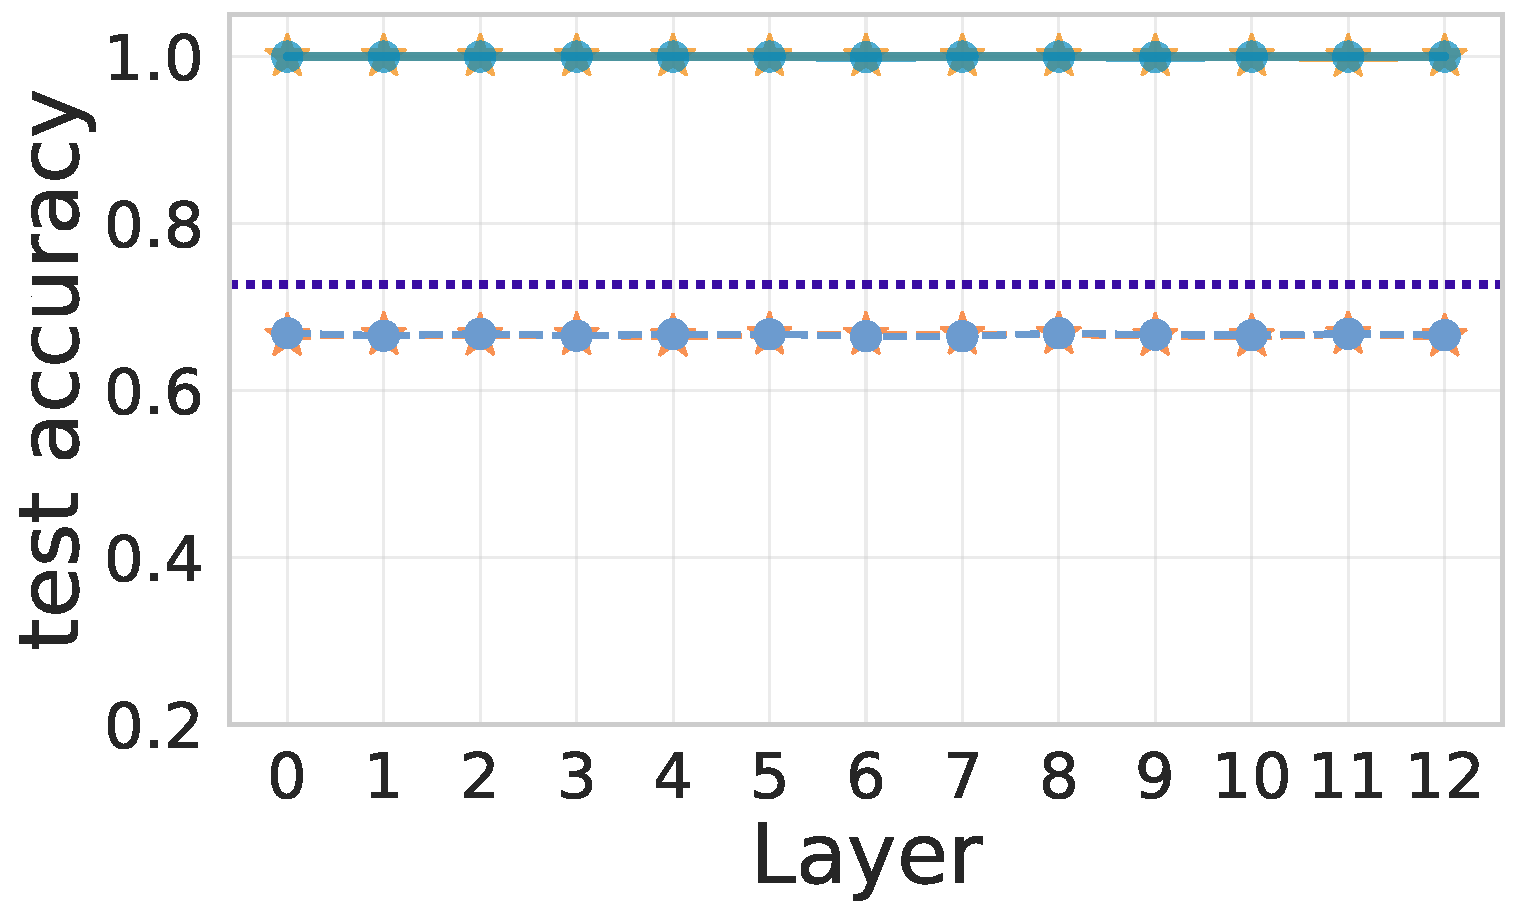
\includegraphics[width=\linewidth]{results_combined/atom_type.pdf}
    \subcaption{atom type}
    \label{fig:acc-atom-type}
\end{subfigure}\hfill
\begin{subfigure}[t]{0.24\textwidth}
    \centering
    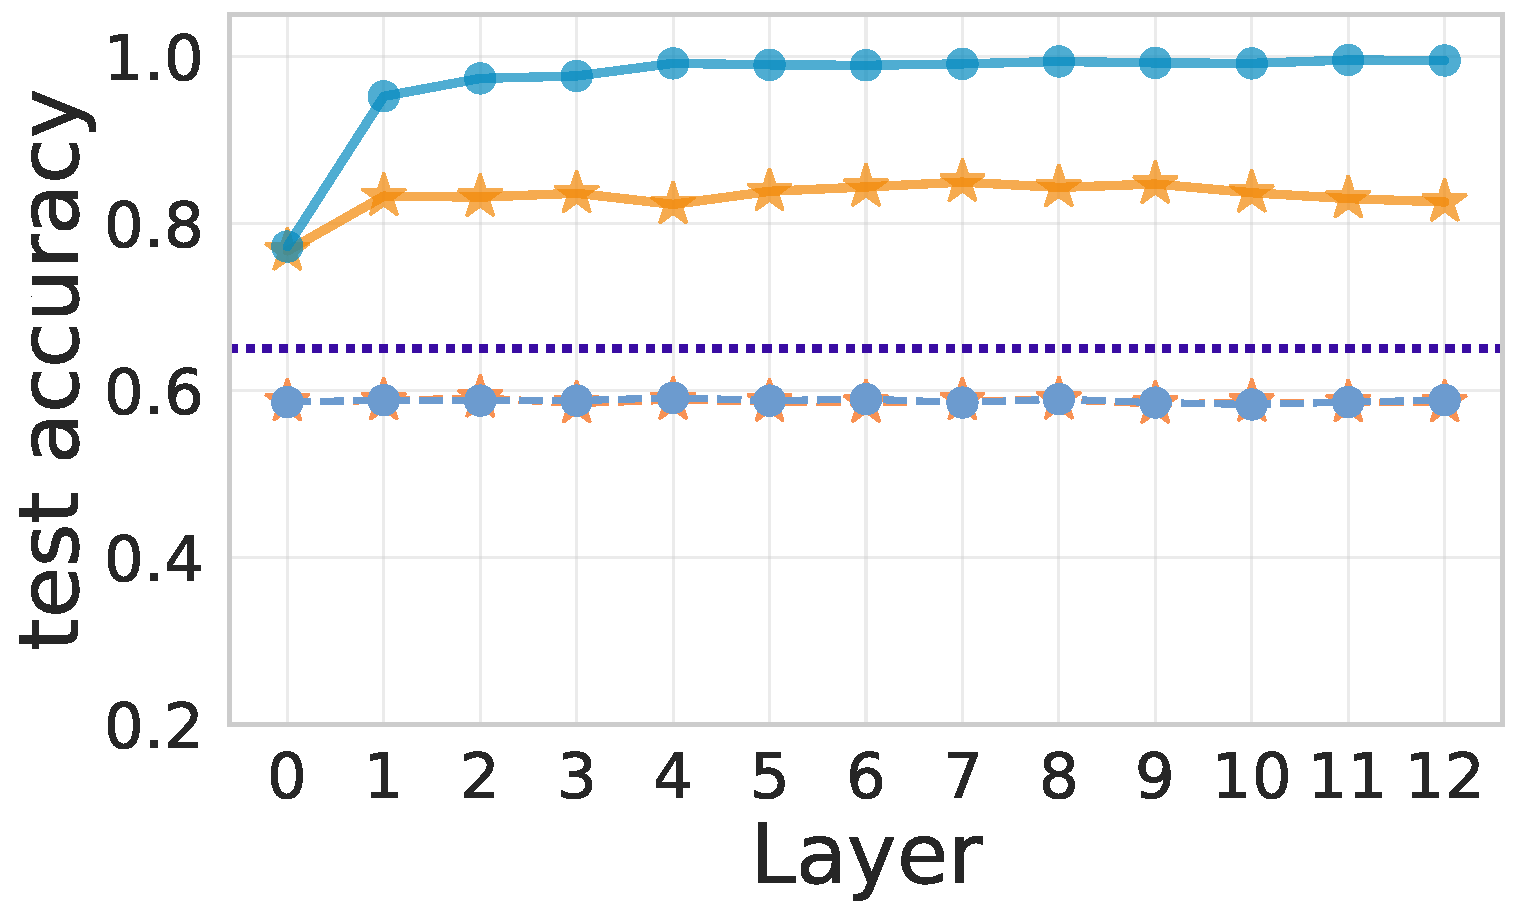
\includegraphics[width=\linewidth]{results_combined/hybridization.pdf}
    \subcaption{hybridization}
    \label{fig:acc-hybridization}
\end{subfigure}\hfill
\begin{subfigure}[t]{0.24\textwidth}
    \centering
    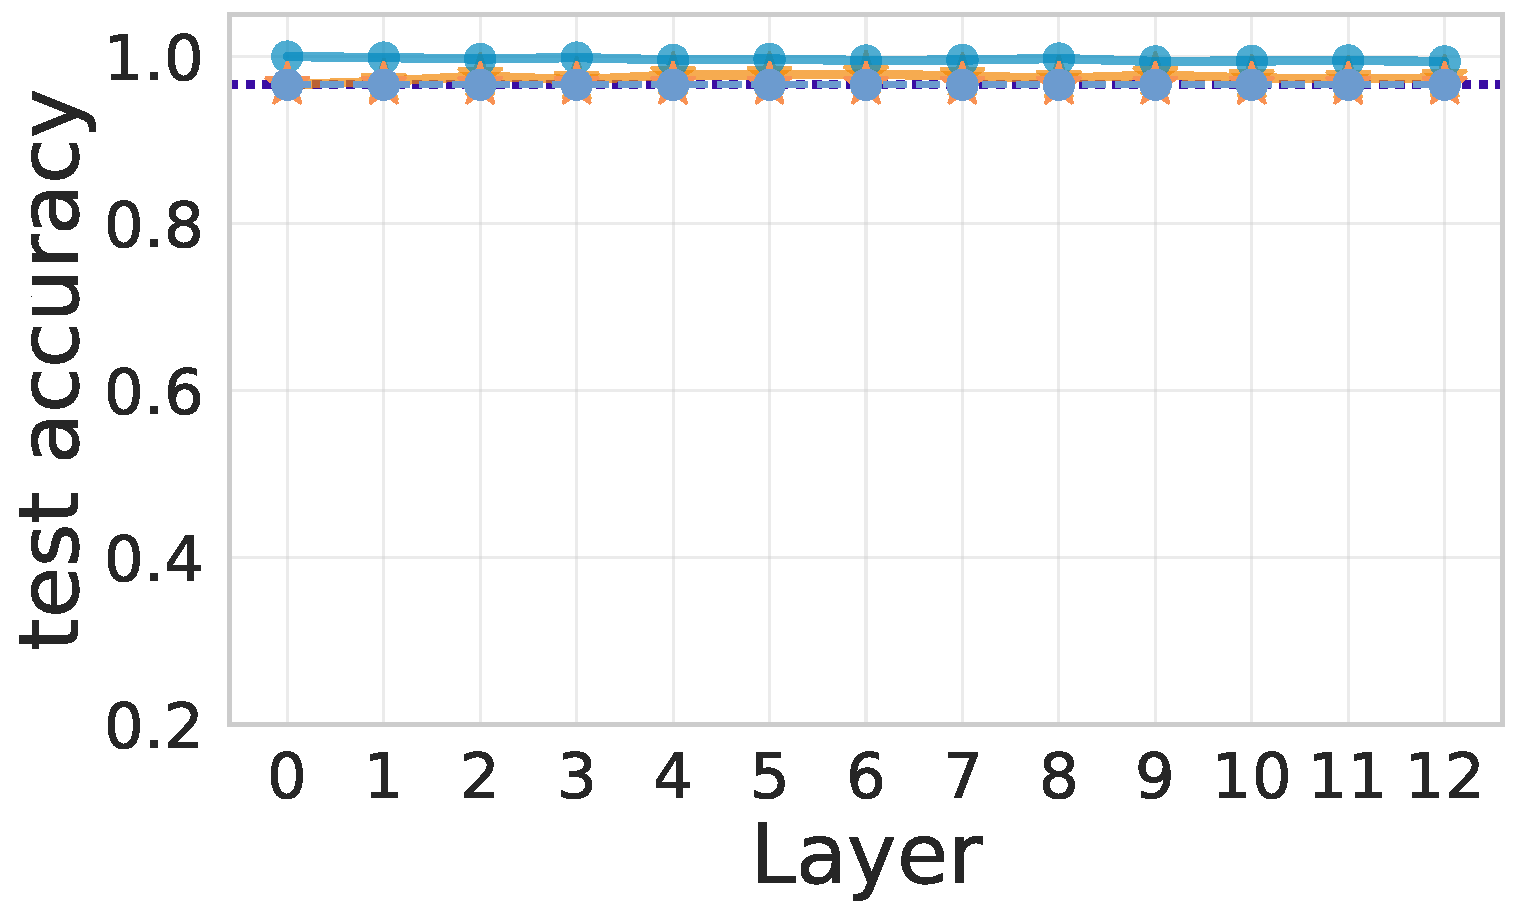
\includegraphics[width=\linewidth]{results_combined/formal_charge.pdf}
    \subcaption{formal charge}
    \label{fig:acc-formal-charge}
\end{subfigure}\hfill
\begin{subfigure}[t]{0.24\textwidth}
    \centering
    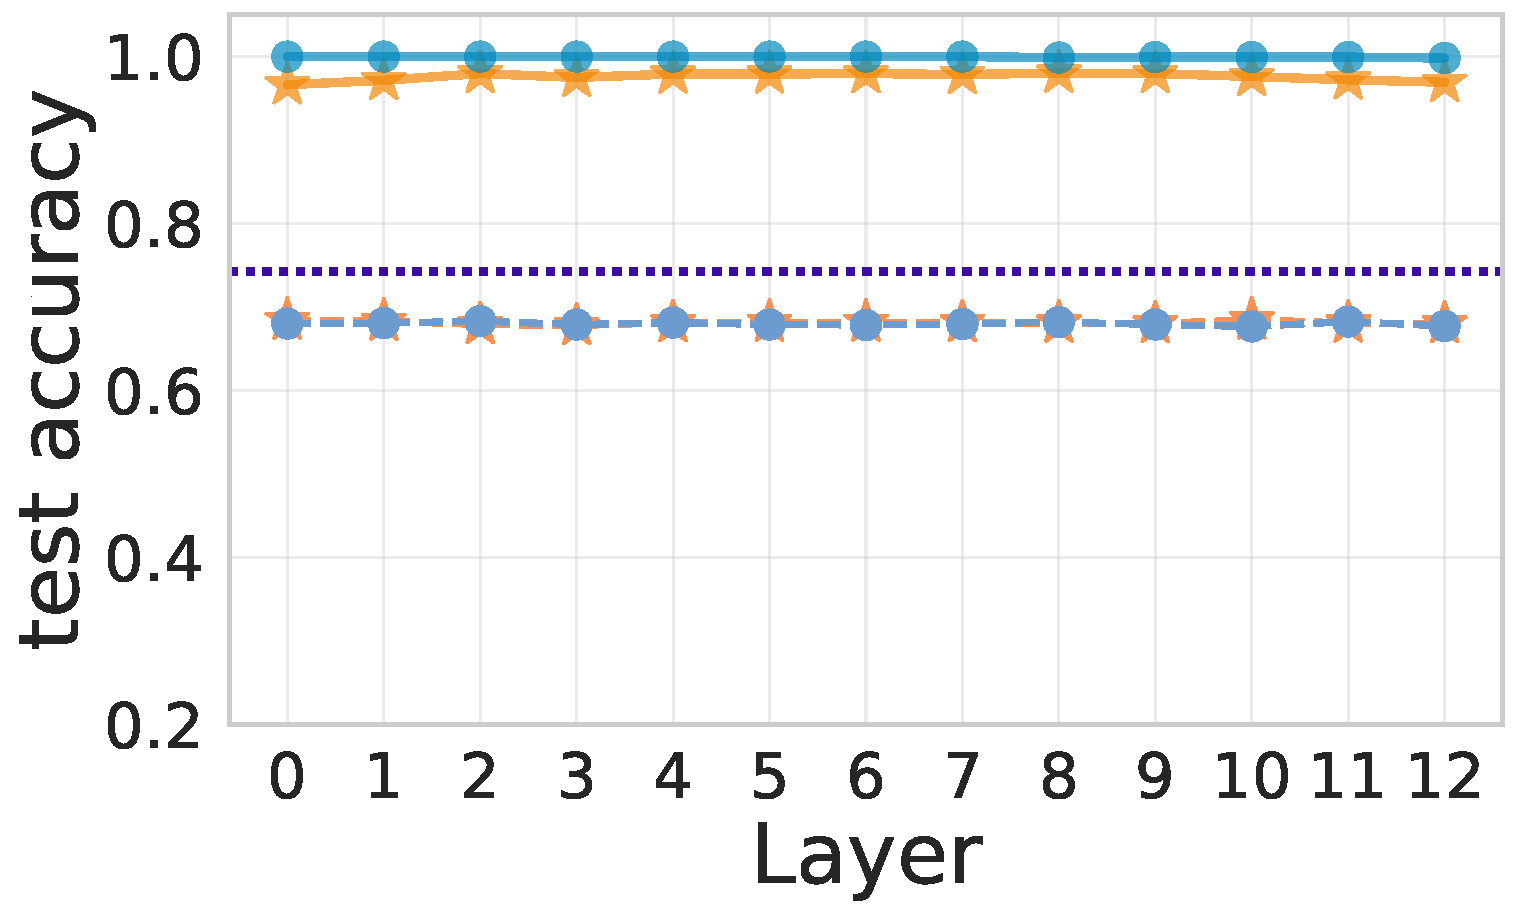
\includegraphics[width=\linewidth]{results_combined/total_valence.pdf}
    \subcaption{total valence}
    \label{fig:acc-total-valence}
\end{subfigure}

\vspace{0.4em}

\centerline{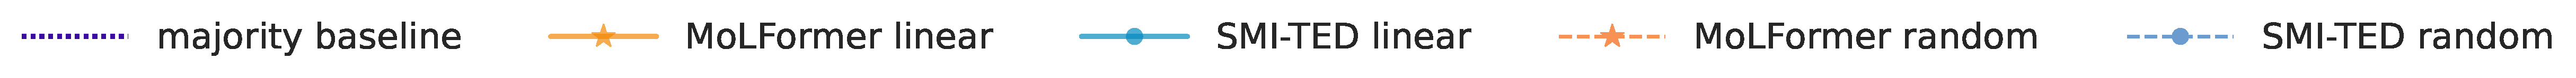
\includegraphics[width=0.9\textwidth]{results_combined/legend.pdf}}

\caption{Linear-probe test accuracy per layer on eight per-atom QM9 properties. \smi reaches near-perfect accuracy by mid-layers on the contextual properties (ring membership, degree, chiral tag, hybridization, total valence), while \molm plateaus several points below; the surface-form properties (atom type, aromaticity) saturate at the embedding in both models.}
\label{fig:acc}
\end{figure*}


\para{Some properties can be read directly from the SMILES string.}
Aromaticity (Figure~\ref{fig:acc-is-aromatic}) reaches $100\%$ test accuracy at layer~$0$ in both \molm and \smi and remains flat across depth. The SMILES tokenizer encodes aromaticity through letter case (lowercase \texttt{c}, \texttt{n}, \texttt{o}, etc.\ for aromatic atoms), so a single token already carries the label; no encoder computation is needed. Atom type and formal charge sit in the same regime: each element symbol is a distinct token, so probe accuracy is at $100\%$ from the embedding for atom type and at $0.97$--$1.00$ for formal charge (the majority class is already $0.97$). Probe accuracy on these tasks reflects tokenizer design rather than learned representation, and we move them to Appendix~\ref{app:probe-all}.

\para{\smi encodes contextual properties more cleanly than \molm.}
The clearest cross-model gap appears on properties that cannot be read from a single SMILES token: ring membership, degree, and chiral tag (Figure~\ref{fig:acc-is-in-ring}, \ref{fig:acc-degree}, \ref{fig:acc-chiral-tag}). The same \texttt{C} token can belong to a ring or not, can have different degree, and can carry different stereochemistry depending on its surroundings, so a probe that achieves high accuracy on these tasks must read information that the encoder put there from context. \smi reaches near-perfect accuracy by mid-layers on all three (and on hybridization in Appendix~\ref{app:probe-all}), while \molm plateaus around $0.85$, $0.85$, $0.85$, and $0.62$, respectively. The MLP probe (Appendix~\ref{app:mlp}) and the random-features control (Appendix~\ref{app:random}) confirm the gap is not an artifact of probe capacity: the MLP probe improves on the linear probe by at most $0.03$ accuracy across all (task, layer) pairs, and random-features probes collapse to majority-class performance. Given the architectures are nearly identical, the difference plausibly stems from pretraining producing more linearly organized representations of context-dependent structure in \smi.

The probe-only conclusion is, however, partial: it locates information but does not show that the encoder uses it. We resolve this in the next subsection.

\subsection{Causal intervention: what is used}
\label{sec:res-steer}
\begin{figure*}[t]
\centering
\begin{subfigure}[t]{0.24\textwidth}
    \centering
    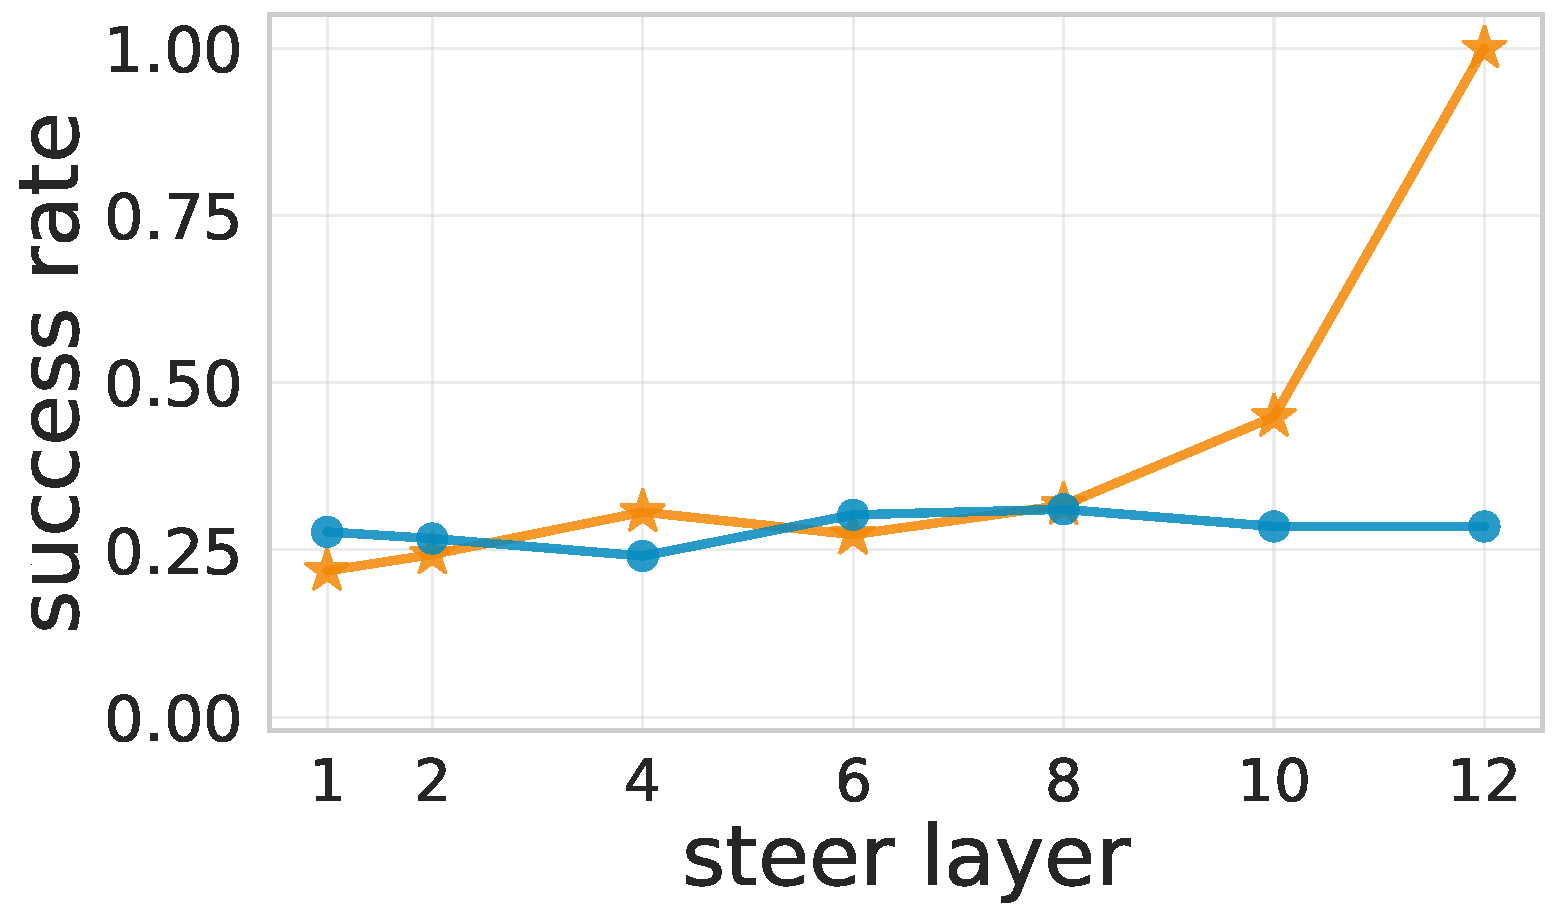
\includegraphics[width=\linewidth]{results_steer_layers/by_layer_atom_type.pdf}
    \subcaption{atom type}
\end{subfigure}\hfill
\begin{subfigure}[t]{0.24\textwidth}
    \centering
    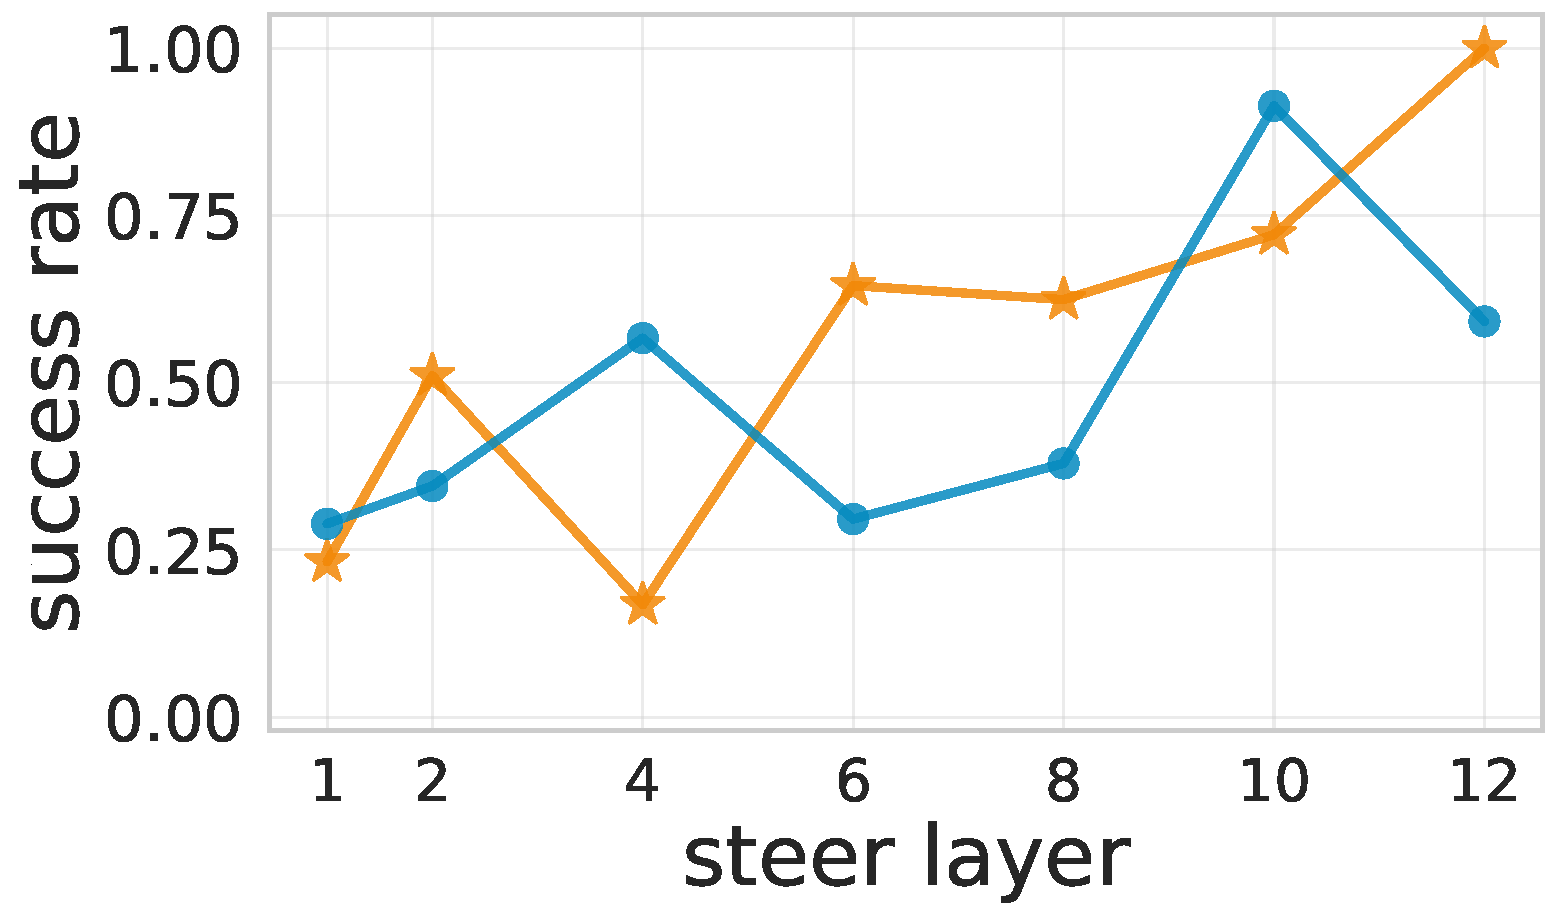
\includegraphics[width=\linewidth]{results_steer_layers/by_layer_hybridization.pdf}
    \subcaption{hybridization}
\end{subfigure}\hfill
\begin{subfigure}[t]{0.24\textwidth}
    \centering
    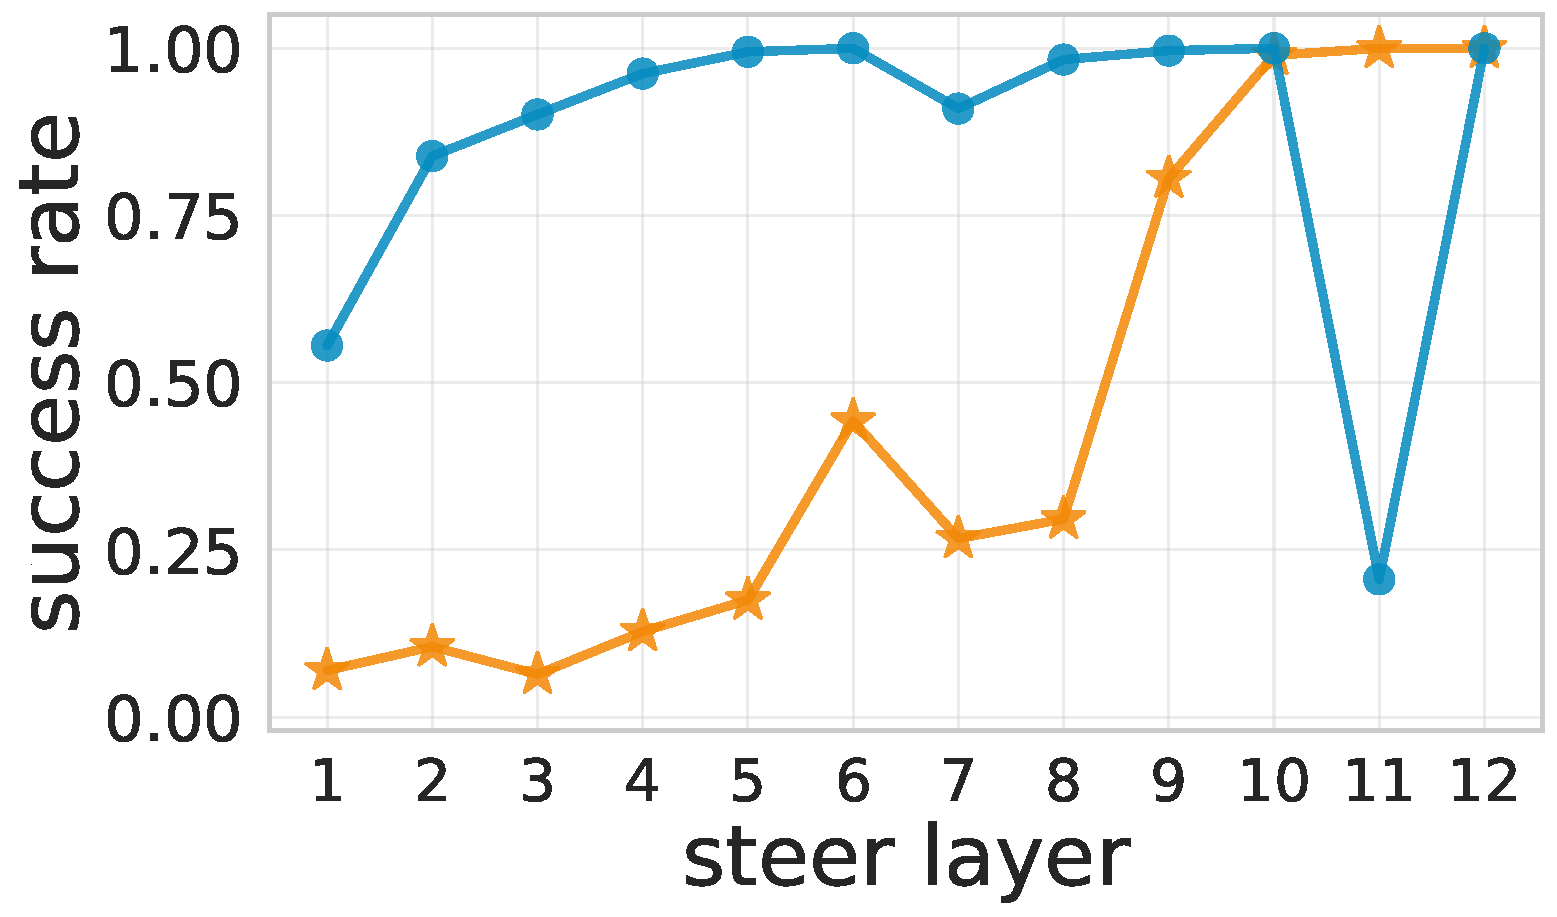
\includegraphics[width=\linewidth]{results_steer_layers/by_layer_chiral_tag.pdf}
    \subcaption{chiral tag}
\end{subfigure}\hfill
\begin{subfigure}[t]{0.24\textwidth}
    \centering
    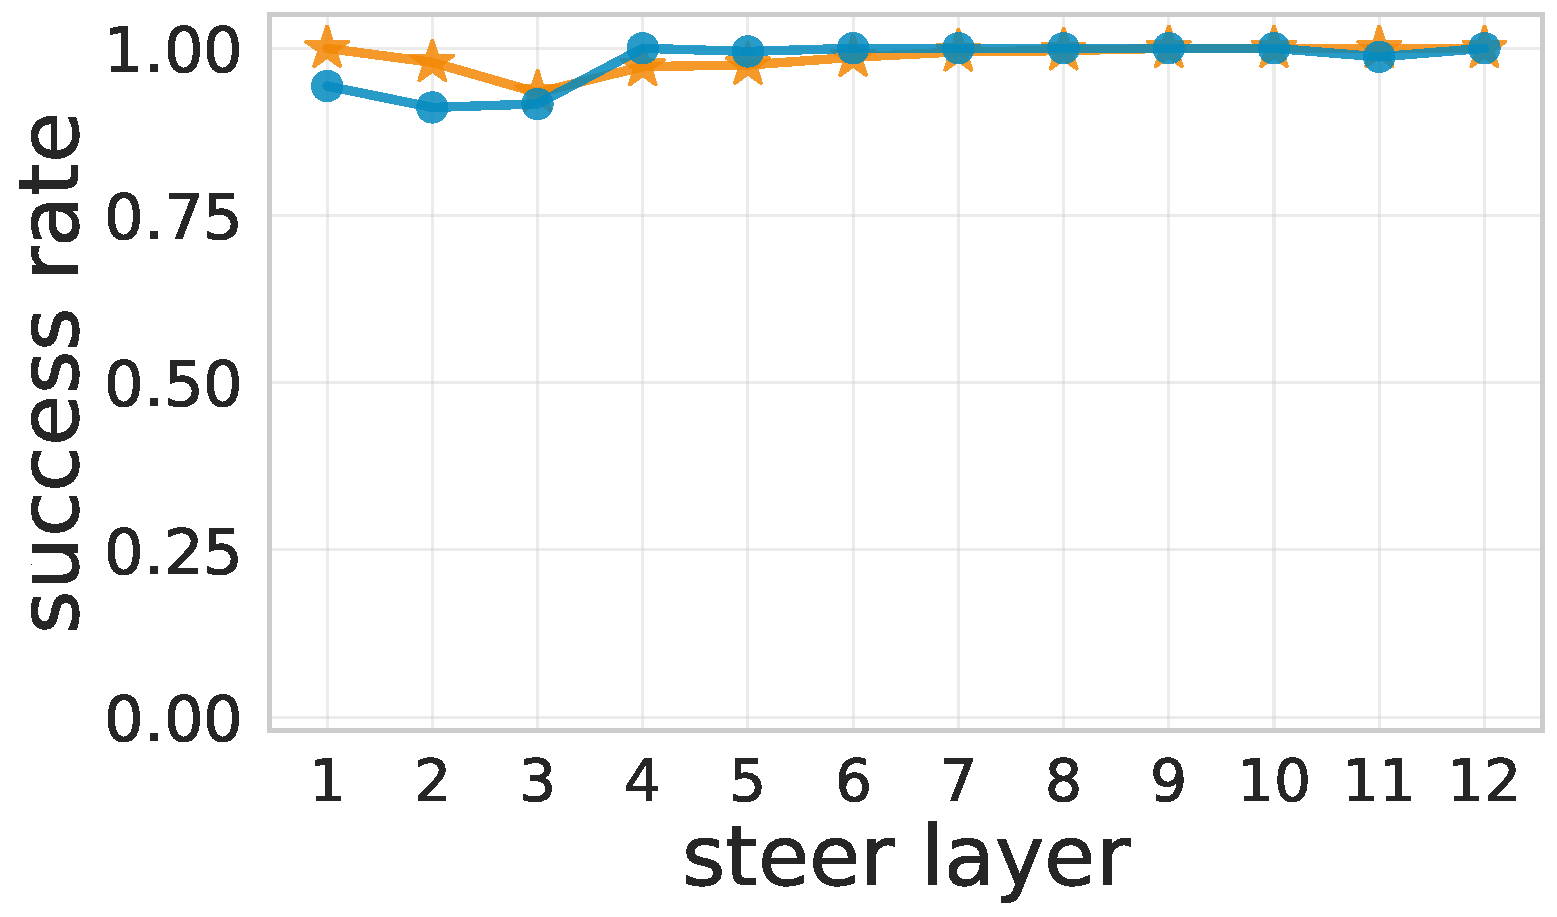
\includegraphics[width=\linewidth]{results_steer_layers/by_layer_is_aromatic.pdf}
    \subcaption{is aromatic}
\end{subfigure}
\vspace{0.6em}

\begin{subfigure}[t]{0.24\textwidth}
    \centering
    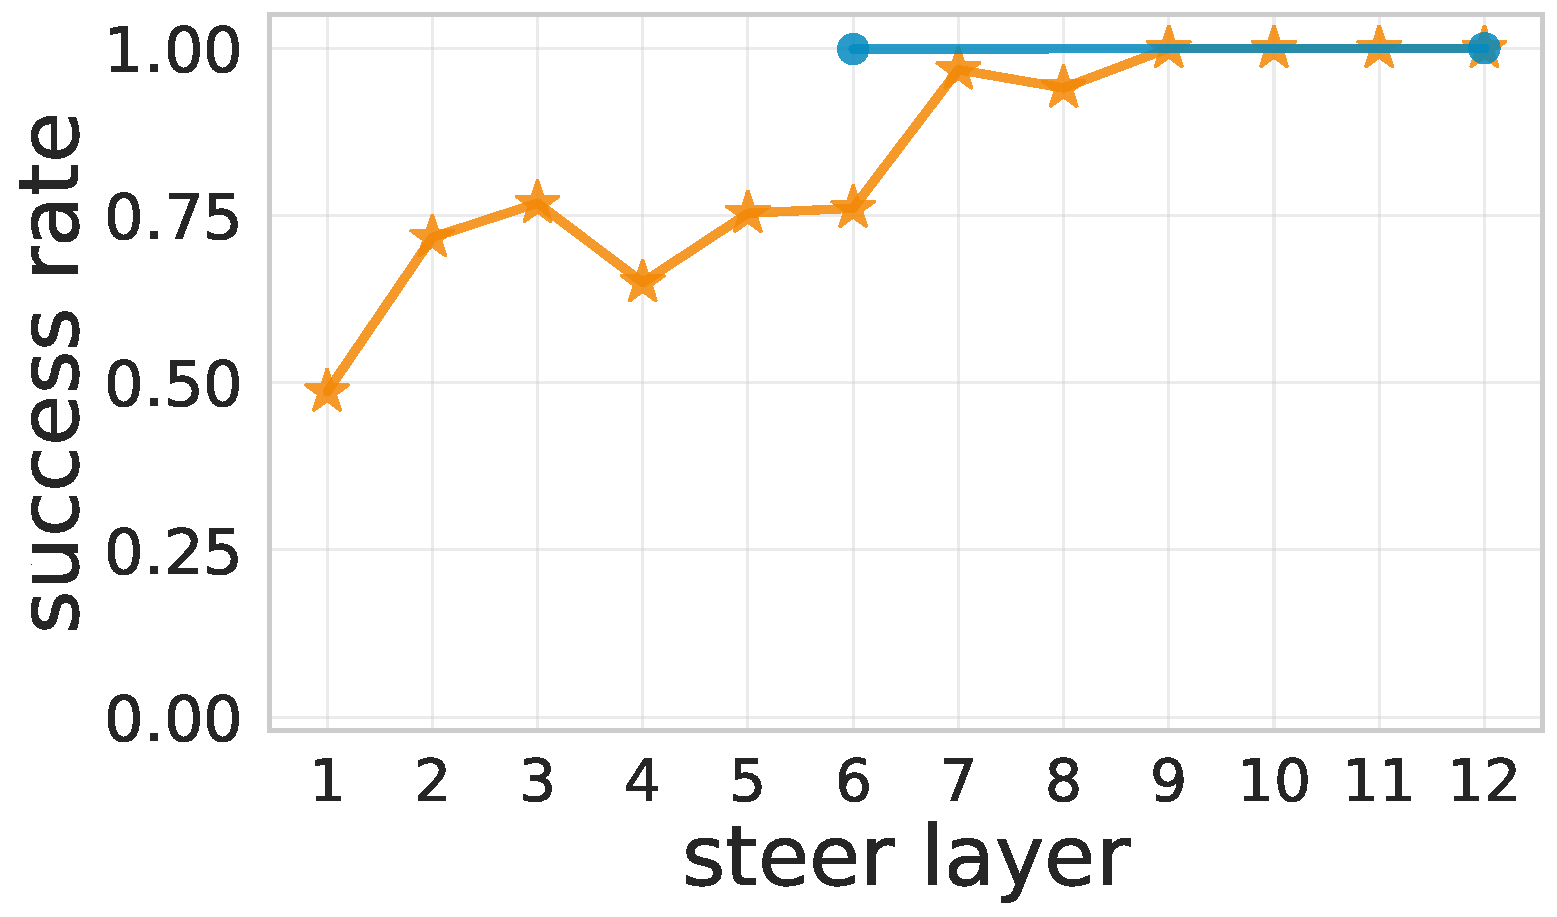
\includegraphics[width=\linewidth]{results_steer_layers/by_layer_is_in_ring.pdf}
    \subcaption{is in ring}
\end{subfigure}\hfill
\begin{subfigure}[t]{0.24\textwidth}
    \centering
    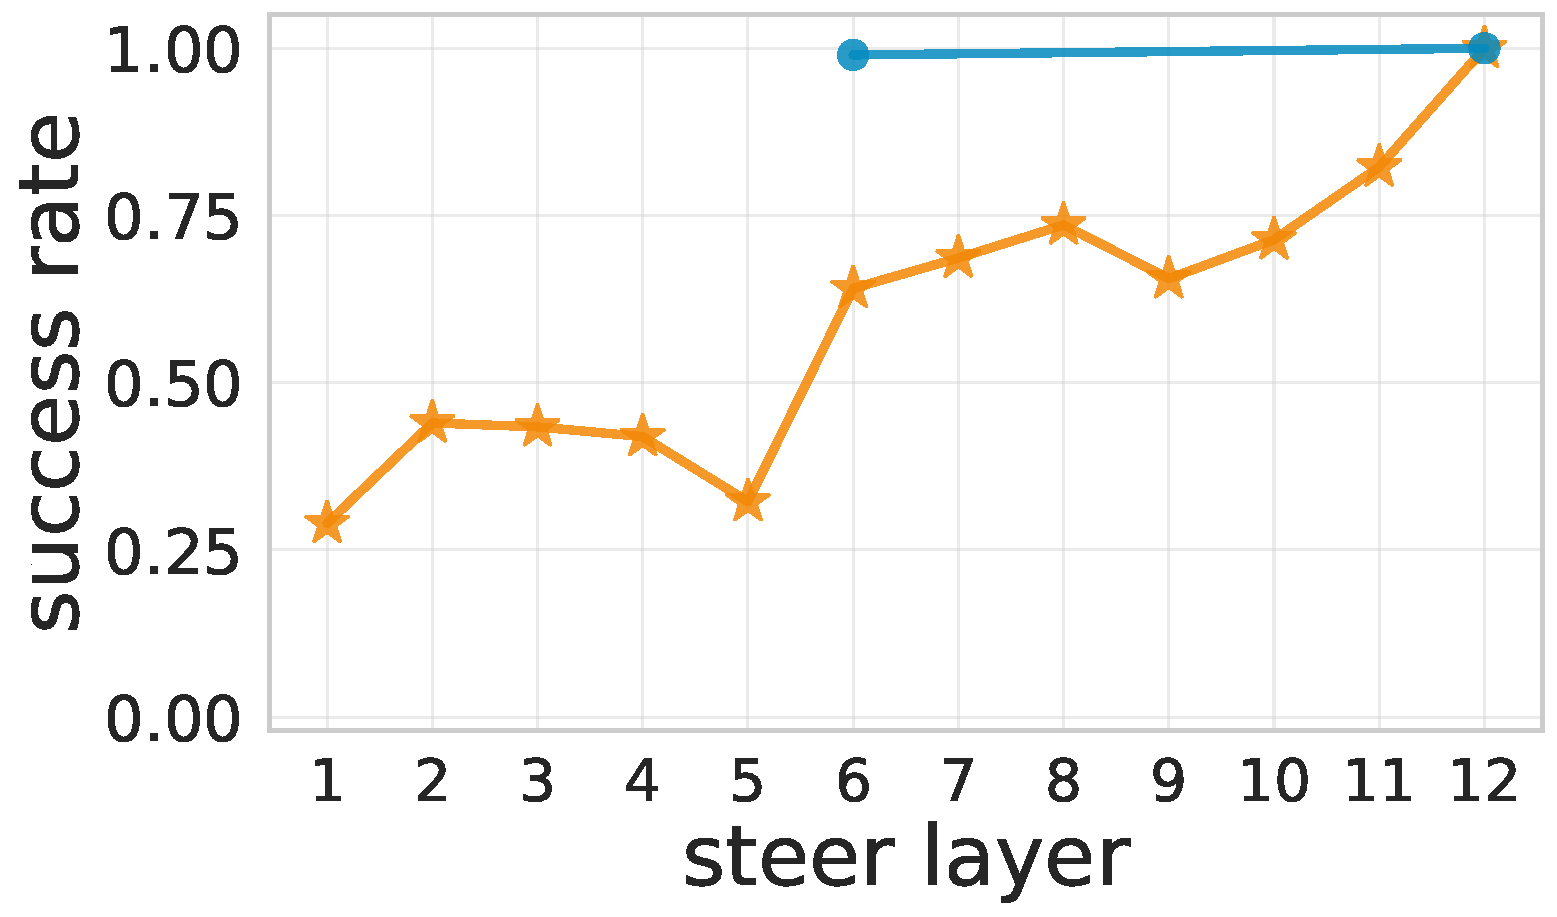
\includegraphics[width=\linewidth]{results_steer_layers/by_layer_degree.pdf}
    \subcaption{degree}
\end{subfigure}\hfill
\begin{subfigure}[t]{0.24\textwidth}
    \centering
    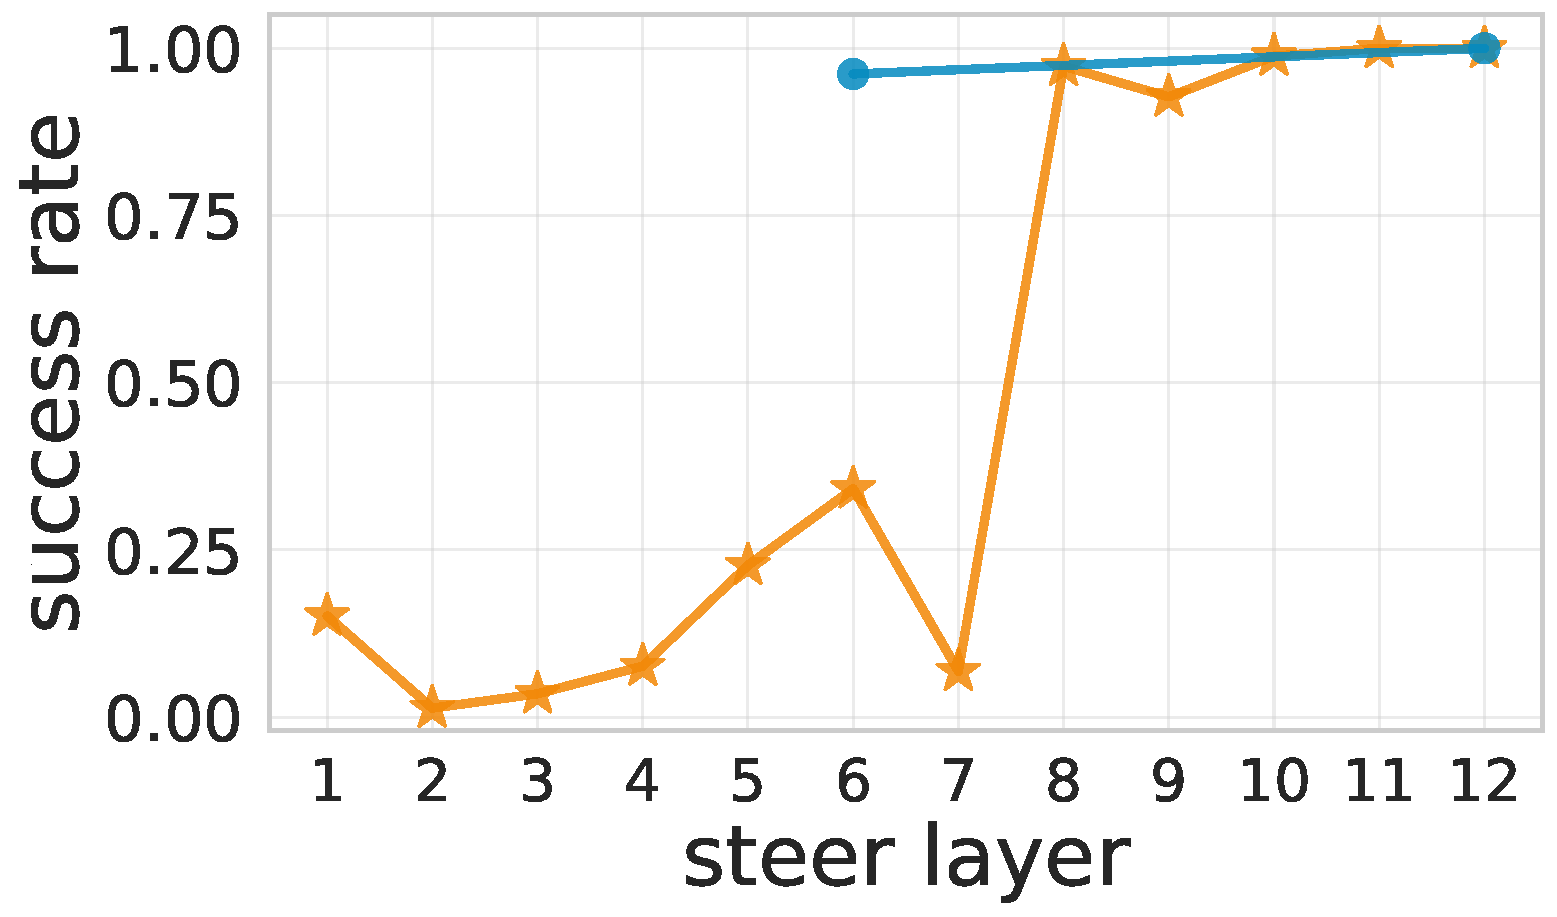
\includegraphics[width=\linewidth]{results_steer_layers/by_layer_formal_charge.pdf}
    \subcaption{formal charge}
\end{subfigure}\hfill
\begin{subfigure}[t]{0.24\textwidth}
    \centering
    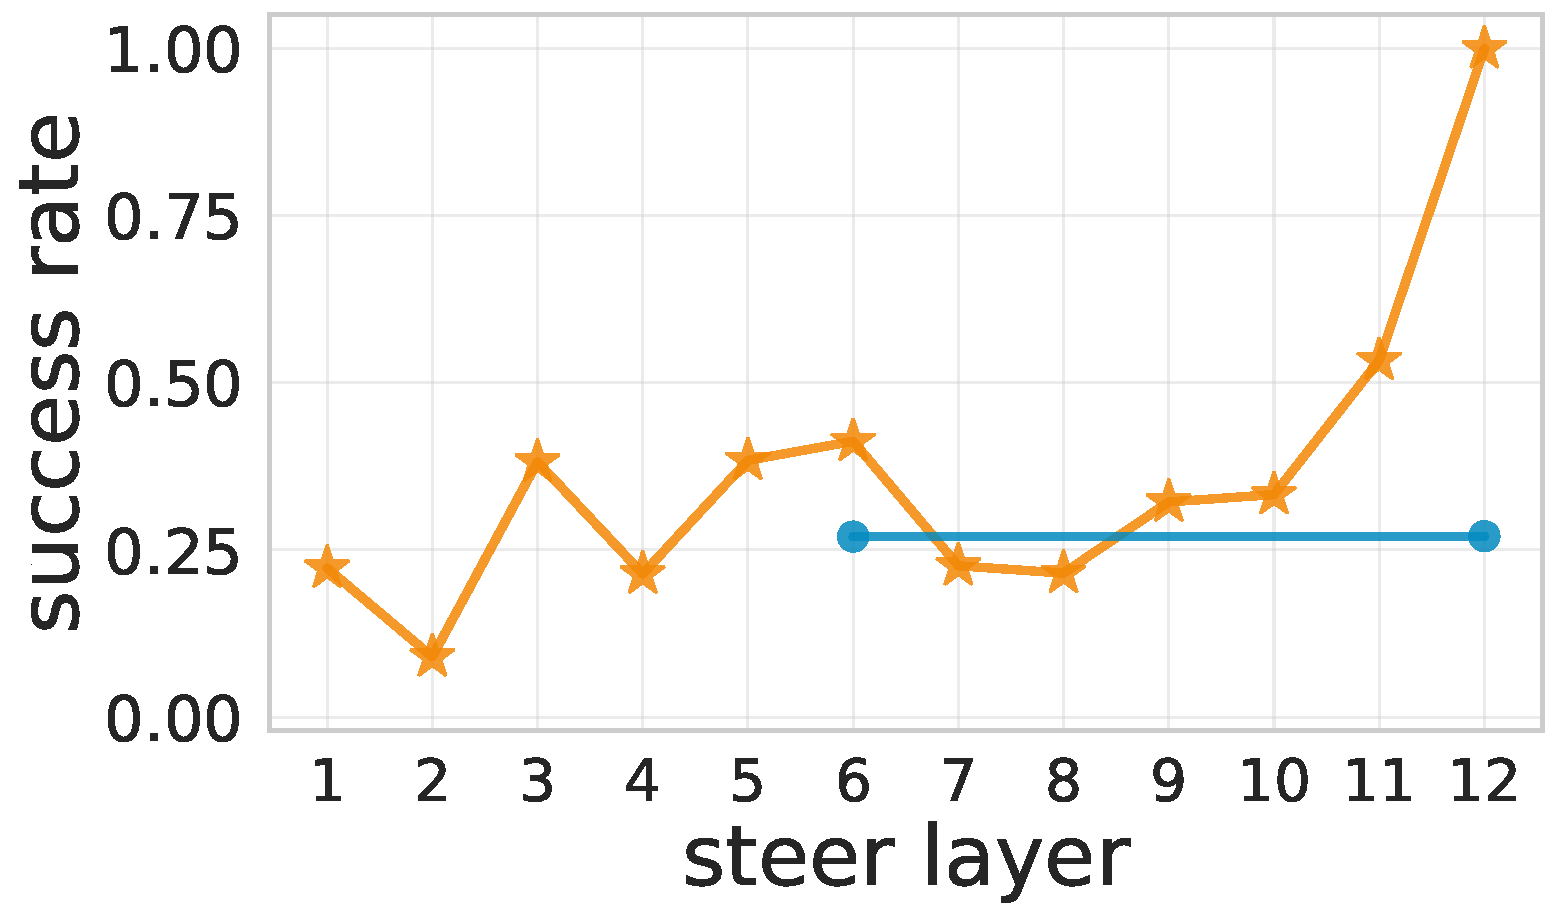
\includegraphics[width=\linewidth]{results_steer_layers/by_layer_total_valence.pdf}
    \subcaption{total valence}
\end{subfigure}

\vspace{0.4em}

\centerline{
\includegraphics[width=0.5\textwidth]{results_steer_layers/by_layer_legend.pdf}}

\caption{\textbf{Intervention success rate as a function of the steer layer.} For each (task, model, layer~$\ell$) we intervene at $\ell$ along the layer-$\ell$ probe direction and read the layer-$12$ probe; the curve plots the best success rate over $\alpha$ on $200$ held-out QM9 molecules. \smi's curve is flat near~$1$ on all binary contextual tasks (ring membership, aromaticity), meaning the probed direction is a usable channel at \emph{every} depth. \molm's ring-membership curve climbs from $\sim 0.5$ at layer~$1$ to $1.00$ by layer~$9$, indicating the information is causally used only at the deepest layers despite being partially decodable throughout. Multi-class tasks (atom type, hybridization, total valence) include a probe-prototype geometry confound on the cycle target and are interpreted with that caveat in the text.}
\label{fig:steer-layer}
\end{figure*}


For each (task, source class $c$, target class $c'$, steer layer $\ell$) we add $\alpha \cdot (\mathbf{W}_{c'}-\mathbf{W}_{c})/\boldsymbol{\sigma}$ at every atom-token position whose baseline prediction is $c$, run the rest of the encoder, and read the layer-$12$ probe; \emph{intervention success rate} is the fraction of those positions whose post-intervention layer-$12$ prediction equals $c'$. For binary tasks $c'$ is the only other class; for multi-class tasks we use a cycle target $c' = (c + 1) \bmod C$. Setup, hook implementation, and the per-source moved-off-source diagnostic are in Appendix~\ref{app:steering}. Single-layer interventions at $\ell{=}6$ already reproduce the probing-level ranking on contextual binary tasks (ring membership: $76\%$ on \molm, $100\%$ on \smi; Table~\ref{tab:steering-success} in Appendix~\ref{app:steering}).

\para{Sweeping the steer layer localizes \emph{where} information is causally used.}
A single-layer intervention can only confirm or deny encoder use at that depth; it cannot say where else the property is causally available. We therefore sweep $\ell \in \{1, \ldots, 12\}$ and report, for each (task, model, $\ell$), the intervention success rate at the best-performing $\alpha$ on the held-out molecules (Figure~\ref{fig:steer-layer}).

\emph{Aromaticity} (Figure~\ref{fig:steer-is-aromatic}) gives the trivial baseline. Probe accuracy is $1.0$ from the embedding and intervention success is $\approx 1.0$ at every depth in both models. The probe direction is a usable channel everywhere because the property essentially \emph{is} the embedding.

\emph{Ring membership} (Figure~\ref{fig:steer-is-in-ring}), \emph{degree} (Figure~\ref{fig:steer-degree}), and \emph{chiral tag} (Figure~\ref{fig:steer-chiral-tag}) all show the same pretraining-difference shape. \smi's success rate climbs rapidly through the early layers and saturates at $1.0$ by mid-depth, in lockstep with the probe reaching near-perfect accuracy: the probed direction is treated as a usable channel by the encoder from mid-layers onward. \molm's success rate, by contrast, climbs gradually and only reaches $1.0$ at the top of the encoder, even though its mid-layer probe accuracy (around $0.85$) is roughly constant across that range. The probe finds a partial linear correlate at every depth in \molm, but only the deepest layers give the encoder a direction that subsequent computation routes through.

\subsection{Discussion: encoded versus used}
\label{sec:res-disc}

The two measurements jointly carve up our observations. When probe accuracy is high \emph{and} intervention success is high---aromaticity at every depth in both models, ring membership / degree / chiral tag at and beyond mid-layers in \smi---the property is both encoded and causally used: it is what the rest of the encoder reads. When neither is high, the property is simply not in the representation; we do not see this case in our eight tasks. The interpretively interesting case is the asymmetry: a probe that decodes the property well at a given depth, but an intervention along the same direction that does not control the layer-$12$ readout. The layer sweep is what makes this case interpretable.

\para{Hypothesis: the information is used at a different depth.}
Under this reading the probe at the intervention layer is reading a passive correlate; the encoder's computational channel for the property lives at another depth, typically deeper. The diagnostic is the layer sweep: the depth at which intervention success becomes high is the depth at which the encoder routes through the probed direction. \molm on degree (Figure~\ref{fig:steer-degree}) is the cleanest instance. Probe accuracy is roughly constant ($\approx 0.85$) across mid-layers but intervention success climbs from $0.29$ at layer~$1$ to $1.00$ at layer~$12$: the information is partially encoded throughout but causally used only at the top of the encoder. Ring membership, formal charge, and chiral tag on \molm follow the same shape (Appendix~\ref{app:steer-all}). This is the form of pretraining gap that probing alone obscures: \molm and \smi have qualitatively similar mid-layer probe accuracies on these tasks within an order of magnitude, but only \smi's representations are organized as a usable channel from mid-depth onward.

\para{Synthesis: \smi's pretraining gap is both representational and functional.}
Combining probing and intervention sharpens the qualitative claim made by prior work~\cite{soares2024smi, sharma2025foundation} that \smi's stronger downstream performance reflects better representations. Probing shows \smi encodes contextual properties as cleaner linear directions than \molm. Intervention shows those same directions are routed through every subsequent encoder block in \smi, whereas \molm's are routed only at the deepest layers. The advantage is therefore not located at any single depth or in either measurement alone: it is the joint property of being both \emph{cleanly organized} and \emph{causally used} throughout the encoder, which is what makes the representations more directly available to downstream heads.
